\documentclass[10pt]{exam}
\usepackage[hon]{template-for-exam}
\usepackage{enumitem}
\usepackage{tikz}
\usepackage{multicol,graphicx,cclicenses}
\usetikzlibrary{shadings,decorations.pathmorphing,arrows.meta,patterns}



\def\mytitle{Chapter 11 (Simple Harmonic Motion \& Waves)}
\author{Rohrbach}
\date{\today}

\def\mymaketitle{
  \begin{flushleft}
    {\LARGE \textbf \mytitle \par}
  \end{flushleft}
}



\begin{document}


\mymaketitle



\newcommand{\stampbox}[1]{

  \hfill
  \begin{tikzpicture}[every text node part/.style={align=center}]
     \node[gray!50,draw,rounded corners] at (0,0) 
      {\sc Stamp \\ \sc Here \\ \small #1 \sc Points};
  \end{tikzpicture}
  \vspace{0.5em}
  
  \hrule

}


%%%%%%%%%%%


\section*{Homework Check A (collected on 11A Mini-Test Day)}

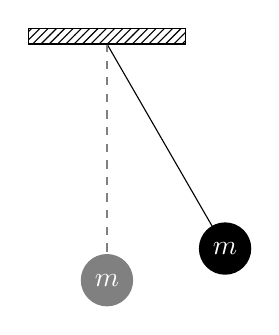
\begin{tikzpicture}
  \def\len{3}
  \draw (0,0) -- (-60:\len) 
    node[circle,fill=black,text=white] (m) {$m$};
  \draw[dashed,gray] (0,0) -- (0,-\len) 
    node[circle,fill=gray,text=white] (m') {$m$};
  \draw[pattern=north east lines] 
    (-1,0) rectangle (1,0.2);
\end{tikzpicture}


%%%%%%%%%%%


\paragraph{Simple Harmonic Motion} pp. 322-323 \#1, 2, 5, 6, 8, 9, 11, 13, 14, 17, 18, 20
\dotfill Complete by March 7

\stampbox{5}

%%%%%%%%%%%

\paragraph{Simple Pendulum} pp. 324-325 \#27, 29, 30, 64
\dotfill Complete by March 11

\stampbox{5}

%%%%%%%%%%%

\paragraph{Conceptual Questions} p. 320-321 \#1, 4, 5, 6, 7
\dotfill Complete by test day
   
{\sc These questions should have at least one full sentence 
      of explanation}

\stampbox{5}

%%%%%%%%%%%%%%

\paragraph{Misconceptual Questions} pp. 321-322 \#1, 2, 3, 6, 7, 8, 
\dotfill Complete by test day
   
{\sc You do not need to get this one stamped,
but these are good review for your test!}

\vspace{0.5em}
\hrule

%%%%%%%%%%%%%%

\paragraph{Bonus Problems!} \#19
\dotfill Turn in separately on test day!

\vspace{0.5em}
\hrule


\paragraph{Mini-Test will be on March 14 ($\pi.2025$)} \hfill

\vspace{0.5em}

\hrule


\section*{Equations}

\begin{align*}
  F_S &= -kx &
  KE &= \frac{1}{2}mv^2 &
  PE_e &= \frac{1}{2}kx^2&
  PE_g &= mgy \\
  f_s &=\frac{1}{2\pi}\sqrt{\frac{k}{m}} &
  f_p &=\frac{1}{2\pi}\sqrt{\frac{g}{L}} &
  \omega &= 2\pi f &
  x(t) &= A \sin\left(\omega t + \phi\right)
\end{align*}


%%%%%%%%%%%

\pagebreak

\section*{Answers}

\begin{multicols}{4}

  \begin{itemize}[noitemsep]
    \item[1.]  0.84 m
    \item[2.]  1.36 Hz
    \item[5.]  $k = 653$ N/m; \\
               $f = 2.63$ Hz; \\
               $A = 2.1$ cm
    \item[6.]  0.14 N/m;  2.83 Hz
    \item[8.]  $x = 0.28\sin (36.0t)$;\\
               $t = 0.04$ s \& 0.13 s
    \item[9.]  2.25 m \& 3.5 m;  \\
               0.25 Hz \& 0.5 Hz; \\
               4 s \& 2 s
    \item[11.]  $A/\sqrt{2}$
    \item[13.]  0.23 sec
    \item[14.]  0.650 m;  1.34 Hz;  \\
                Total = 17.2 J; \\
                PE = 5.26 J; \\
                KE = 11.92 J
    \item[17.]  $\sqrt{3}$
    \item[18.]  59 N/m;  0.060 J
    \item[20.]  5.5 cm;  0.59 m/s
    \item[27.]  3.0 sec
    \item[29.]  1.8 sec;  0.56 Hz
    \item[30.]  1.4 sec
    \item[64.]  (a) 0.59 Hz;  \\
                (b) 0.55 m/s;  \\
                (c) 0.046 J
    
  \end{itemize}
  
\end{multicols}


\subsection*{Misconceptual Answers}

\begin{multicols}{6}

  \begin{itemize}[noitemsep]
    \item[1.] E
    \item[2.]  A, C, D
    \item[3.]  C
    \item[6.]  E
    \item[7.]  C
    \item[8.]  A
  
  \end{itemize}  
\end{multicols}



%%%%%%%%%%%

\pagebreak

\section*{Homework Check B (collected on 11B Mini-Test Day)}

\begin{center}
  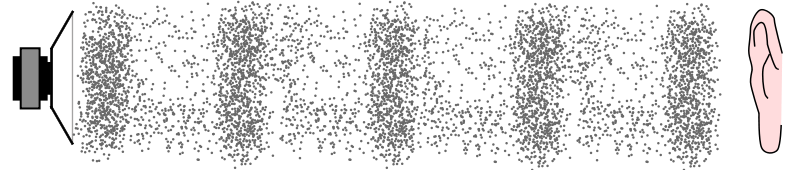
\includegraphics[width=10cm]{sound-wave.png}
\end{center}

\paragraph{Waves} p. 324 \#35, 36, 38
\dotfill Complete by Apr 8

\stampbox{2}

%%%%%%%%%%%

\paragraph{Standing Waves, Resonance} pp. 324-325 \#49, 51, 52
\dotfill Complete by Apr 10

\stampbox{3}

%%%%%%%%%%%

\paragraph{Interference; Beats (From Ch 12)} p. 355  \#46, 47
\dotfill Complete by Apr 11

\stampbox{2}


%%%%%%%%%%%

\paragraph{Conceptual Questions}
\dotfill Complete by test day
   

Ch 11 (pp. 320-321) \#13, 22

Ch 12 (p. 353) \#5, 11, 13, 14, 17

\stampbox{3}

%%%%%%%%%%%%%%

\paragraph{Misconceptual Questions}
\dotfill Complete by test day

Ch 11 (pp. 321-322) \#10, 11, 12, 15

Ch 12 (p. 353) \#12, 13
   
{\sc You do not need to get this one stamped,
but these are good review for your test!}

\vspace{0.5em}
\hrule

%%%%%%%%%%%%%%

\paragraph{Bonus Problems!} \#39
\dotfill Turn in separately on test day!

\vspace{0.5em}
\hrule


\paragraph{Mini-Test will be on Mon, Apr 14} \hfill

\vspace{0.5em}

\hrule


\section*{Equations}

\begin{align*}
  v &= f \lambda &
  f_n &= \frac{nv}{2L} = nf_1 &
  f_{BEAT} &= \left|f_1-f_2\right| %s\\
  %f' &= f\left( \frac{v_{snd}\pm v_{obs}}{v_{snd}\mp v_{src}} \right) &&&
  %v_{snd} &= 343~\text{m/s at 20$^\circ$C}
\end{align*}


%%%%%%%%%%%

\pagebreak

\section*{Answers}

\begin{multicols}{2}

  \begin{itemize}[noitemsep]
    \item[35.]  2.3 m/s
    \item[36.]  1.22 m
    \item[38.]  190 m to 545 m; 
                2.8 m to 3.4 m
    \item[49.]  440 Hz; 880 Hz; 
                132 Hz; 1760 Hz
    \item[51.]  60 Hz; 120 Hz; 180 Hz
    \item[52.]  0.102 m
    \item[46.]  0.5 Hz
    \item[47.]  18.5 kHz or 28.5 kHz
    
  \end{itemize}
  
\end{multicols}


\subsection*{Misconceptual Answers (Ch 11)}

\begin{multicols}{4}

  \begin{itemize}[noitemsep]
    \item[1. ] E
    \item[2. ] A, C, D
    \item[3. ] C
    \item[6. ] E
    \item[7. ] C
    \item[8. ] A
    \item[10.]  A
    \item[11.]  D
    \item[12.]  D
    \item[15.]  A
     
  \end{itemize}  
\end{multicols}

\subsection*{Misconceptual Answers (Ch 12)}

\begin{multicols}{4}

  \begin{itemize}[noitemsep]
    \item[2.]  D
    \item[7.]  E
    \item[8.]  E
    \item[9.]  C
  \end{itemize}  
\end{multicols}





\end{document}